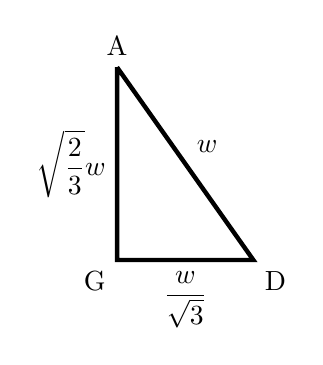
\begin{tikzpicture}[xscale=3, yscale=3, ultra thick]
	%頂点
	\path (0, 0.816) coordinate (A);
	\path (0, 0) coordinate (G);
	\path (0.577, 0) coordinate (D);
	\draw (A) node [above]{A};
	\draw (G) node [below left]{G};
	\draw (D) node [below right]{D};
	%辺
	\draw (A)--(G)--(D)--(A);
	%大きさ
	%
	\path (0, 0.408) node [left]{$\displaystyle\sqrt{\frac{2}{3}}w$};
	\path (0.289, 0) node [below]{$\displaystyle\frac{w}{\sqrt{3}}$};
	\path (0.289, 0.408) node [above right]{$\displaystyle w$};
\end{tikzpicture}
